\documentclass{article}
\usepackage[superscript]{cite}   % remove to use brackets instead of superscripts in citations
\usepackage{graphicx}
\usepackage{fancyhdr}
\usepackage{xcolor}
\usepackage{indentfirst}
\usepackage[a4paper, portrait, margin=1in]{geometry}
\usepackage{lastpage}
\usepackage{float}
\pagestyle{fancy}
\fancyhf{}
\fancyhead[L]{Vupiter}
\fancyhead[R]{Project Proposal}
\rfoot{Page \thepage \hspace{1pt} of \pageref*{LastPage}}
\pagenumbering{arabic}

\usepackage[pdftex,bookmarks,pdfpagemode=UseOutlines,
    pdfauthor={Vupiter Team},
    pdftitle={Project Proposal},colorlinks=true, linkcolor=blue]{hyperref}
% removed colorlinks after bookmarks

\newcommand{\code}[1]{\texttt{\smaller #1}}

\setlength\parindent{5ex}
\setlength\parskip{2ex}

\newcommand{\fig}[1]{\centerline{\includegraphics{#1}}}

\DeclareGraphicsExtensions{.pdf, .jpg, .png}
%\setkeys{Gin}{width=0.85\textwidth}
\begin{document}
\begin{titlepage}
    \begin{center}
        \vspace*{1cm}
            
        \Huge
        \textbf{Vupiter DC Power Supply}
            
        \vspace{0.5cm}
        \LARGE
        Date: \today
            
        \vspace{4.5cm}

        \textbf{Senior Design Project Proposal}
        
        \vspace{1cm}

        \textbf{Team Members:}\\
        Chase Flatau\\
        Alex Jones\\
        Rice Shelley\\
        Al Spies
        \vfill
            
            
        \vspace{0.8cm}
            
        
\includegraphics[width=0.4\textwidth]{university}
            
        \Large

        \textbf{Auburn University}\\
        Department of Electrical and Computer Engineering\\

            
    \end{center}
\end{titlepage}

\tableofcontents
\pagebreak

\section{Project Description}
\par
DC power supplies are easily one of the most important pieces of test equipment 
in a lab while simultaneously being the most basic in concept. The focus of the 
Vupiter project will be to create a low-cost open-source versatile benchtop power 
supply. To make Vupiter versatile we will provide a computer interface that will 
allow power users to automate testing and data collection, in addition to the 
typical front-panel control. This computer interface will allow Vupiter to be 
useful in a much larger domain of experimentation than could be explored with it. 
Community expansion on this computer interface and the design as a whole will be 
enabled through thorough documentation at every stage. We will be documenting not 
just the technical details but also the decision making process along the way meaning 
Vupiter will be able to serve simultaneously as a useful lab tool and as a teaching 
tool. This level of documentation is the critical element frequently missing from most 
open source hardware projects, even other open source supplies, that prevents them 
from becoming truly community projects.
\section{Technical Description}
The design of the Vupiter lab power supply takes in to consideration usability, 
safety, and economic feasibility.  The Vupiter lab power supply will offer 
three independent channels controllable with a physical front panel. In addition 
to the physical control panel PC control will also be provide facilitated by a 
USB interface. The affordability of the design is addressed via choosing cheap 
yet powerful micro-controllers and designing a front panel that is usable yet 
economical.

\subsection{Power Stages}
Benchtop power supplies are frequently attached to sensitive and poorly 
characterized devices meaning that the supply is subject to more rigorous 
and varied performance requirements than a typical specialized supply. 
These performance requirements can be roughly broken down into output noise 
and output step response requirements. These two criteria will be considered 
in addition to our budgetary and environmental requirements when evaluating 
designs. Four topologies for the power supply section of this project are 
explored and explained below, addressing these criteria. The final tallying 
of their pros and cons can be seen in Table X.

\subsubsection{Topology 1 - Linear mode devices only}
This topology is by far the simplest as all it does is transform and rectify mains 
voltage, and then burn any excess voltage as heat in order to control the final 
output voltages. This results in a very high quality output, as there are no elements 
injecting noise and the entire voltage range is available for step response. 
Those benefits are exactly its downfall sadly, as the requirement on the transformer 
for it to work at 60 Hz requires that cycle by cycle it must be able to store a 
large amount of energy in the H-field. This implies a physically large design, as 
the more energy that needs to be stored, the greater the amount of ferrous core needed. 
Not only does this make for bulky and heavy transformers, but it also greatly increases 
the cost. Aside from this, the linear element also has issues, shown in the diagram 
in red. As we cannot adjust the output of the rectifier, that linear element has to 
turn all the excess voltage into heat. This means that the power supply running at 
a low voltage output but drawing high amperage would need to dissipate nearly 200 
Watts would undoubtedly require heat sinking and active cooling, also driving up 
the price and weight of the power supply.

\begin{figure}[H]
    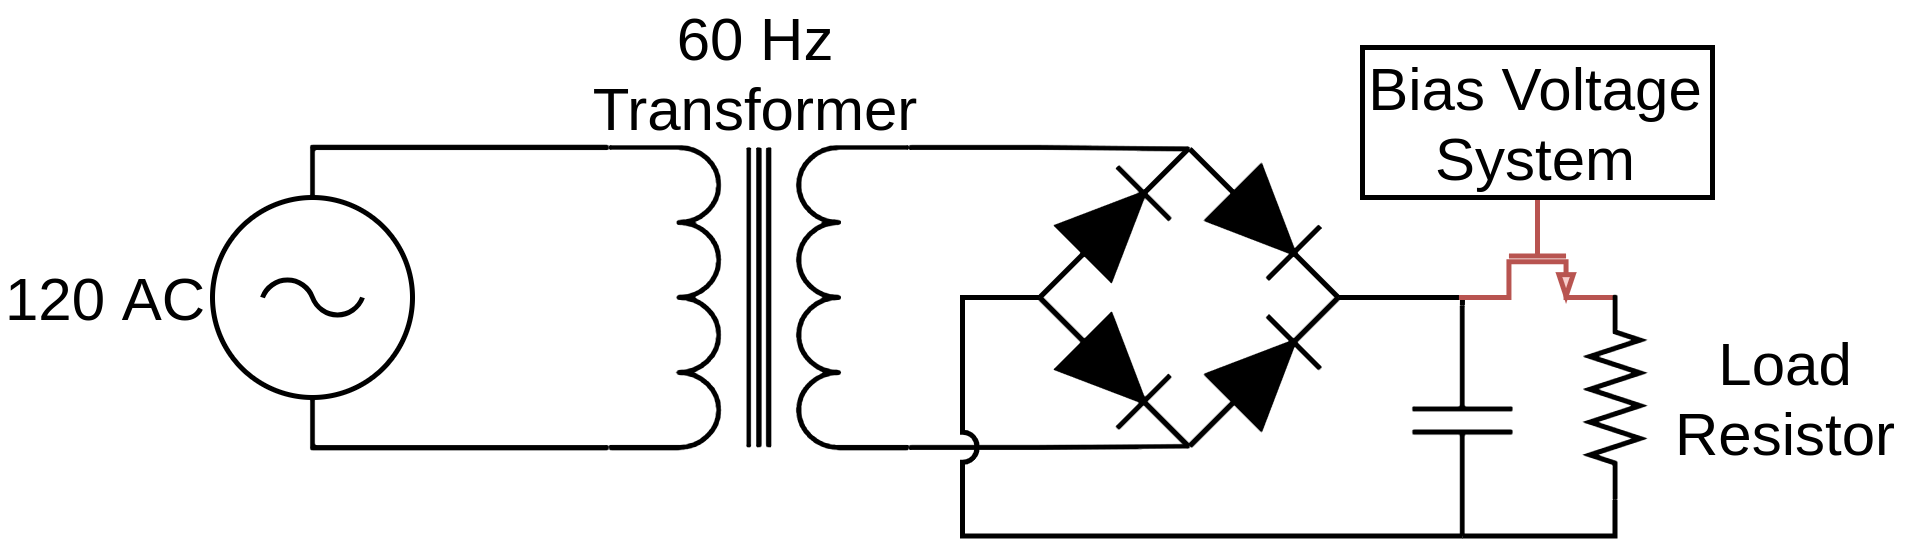
\includegraphics[width=\textwidth]{linear}
    \caption{Entirely linear mode design}
    \label{fig:linear}
\end{figure}

\subsubsection{Topology 2 - Switch mode devices only}
To address the issues with linear regulation, let's examine a purely switch mode 
regulator. As can be seen in Figure 2, line voltage is immediately rectified. 
This gives us an approximately 300V DC supply. From that 300V supply, we switch 
it at high frequency through a transformer. Due to this ability to increase the 
frequency, we can decrease the size and price of the transformer drastically. From 
the output we have to rectify again, and then we go on to our final regulation stage 
which is a buck converter. This buck converter is able to control the output voltage 
at high efficiency, but due to its requirement for high output capacitance, current 
limiting and voltage recovery speed suffer. Even worse, the buck converter both 
fails to filter noise from the first switched converter stage, and also injects 
noise at its switching frequency. This noise, and the poor current limiting results 
in a low quality output that would make this power supply useless in a large number 
of applications. That being said, this design has a low cost and extremely high 
efficiency,as no part of it is dissipating power intentionally, allowing it to 
reduce the size of some parts and completely eliminating other items such as heat 
sinks and fans.

\begin{figure}[H]
    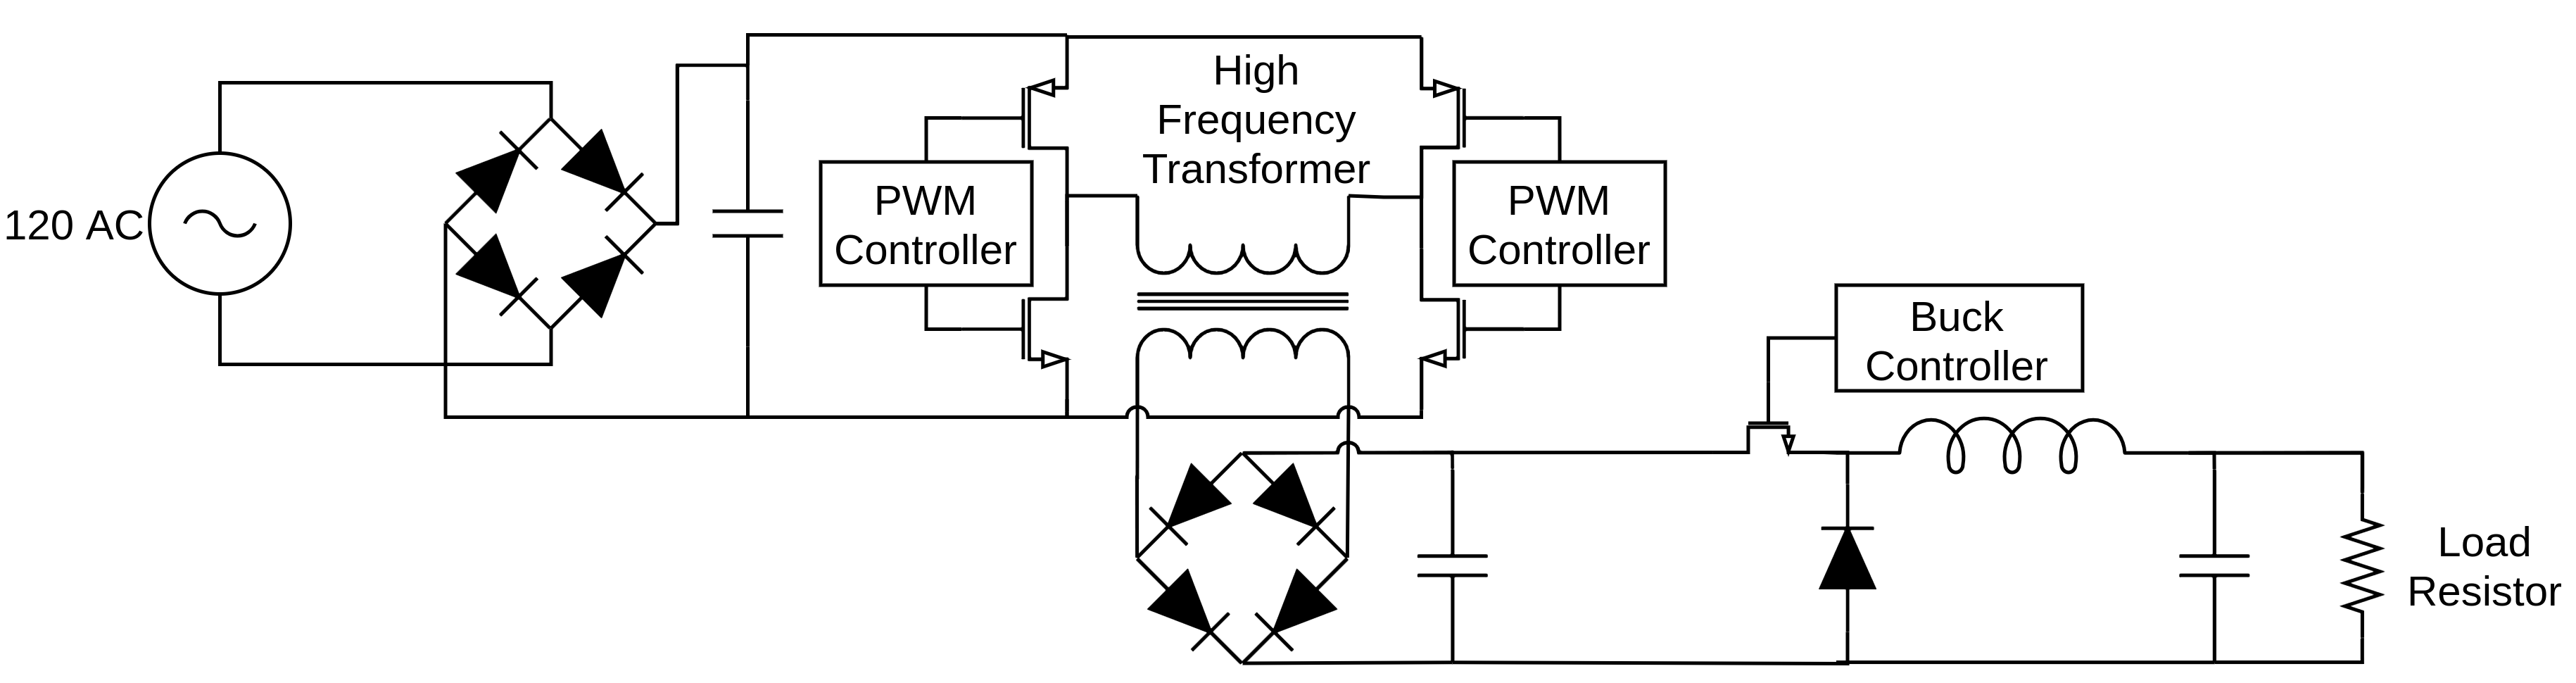
\includegraphics[width=\textwidth]{switched}
    \caption{Entirely switch mode design}
    \label{fig:switched}
\end{figure}
\subsubsection{Topologies 3 and 4 - Mixed mode supplies}

These two topologies are together as they share a single concept and block diagram, 
but there are major differences in their feedback loops and how they respond. 
As can be seen in \autoref{fig:mixed}, these topologies are composed of different pieces 
from topologies one and two, earning them their name as mixed mode rather than 
linear or switch exclusively. These two are using the high frequency transformer 
stage from the switch mode design, followed by a linear regulator on the output. 
This allows us to eliminate the high cost 60 Hz transformer while still maintaining 
the benefits of linear regulation. The switch mode elements here still inject noise, 
but as they are followed by a linear stage, that noise can be filtered both by passive 
elements and by the linear elements, ensuring a high quality output regulation.  

The first of our two topologies in this domain is a fixed mixed mode design. 
This means that the voltage output of the second rectifier is controlled to a 
fixed value, I.E. if the desired voltage is 20V, the transformer will target 25V 
and allow the additional 5V to be dissipated in the linear stage. The benefit 
here is higher efficiency than the linear only design as we can decrease the supply 
voltage at low output voltages while still maintaining strong regulation. 

The alternative to this is a floating mixed mode design whereby the output of the 
second rectifier is regulated to always be just slightly above the dropout of the 
linear stage. This ensures exceptionally high efficiency as the linear element is 
dissipating at most 10 watts even with a short circuit across its output. Where this 
is problematic is when reacting to large step inputs both on the load or the command 
side, as the maximum positive output voltage slew is dictated by the switched elements 
rather than the linear elements which can react almost instantly. Another point off 
for this design is the difficulty of designing a floating switch mode section. This 
can drastically complicate feedback loops and if done improperly will result in an 
unstable output. Due to this, floating output voltages are infrequent, driving up 
the cost to design one as controller IC choice is limited.

\begin{figure}[H]
    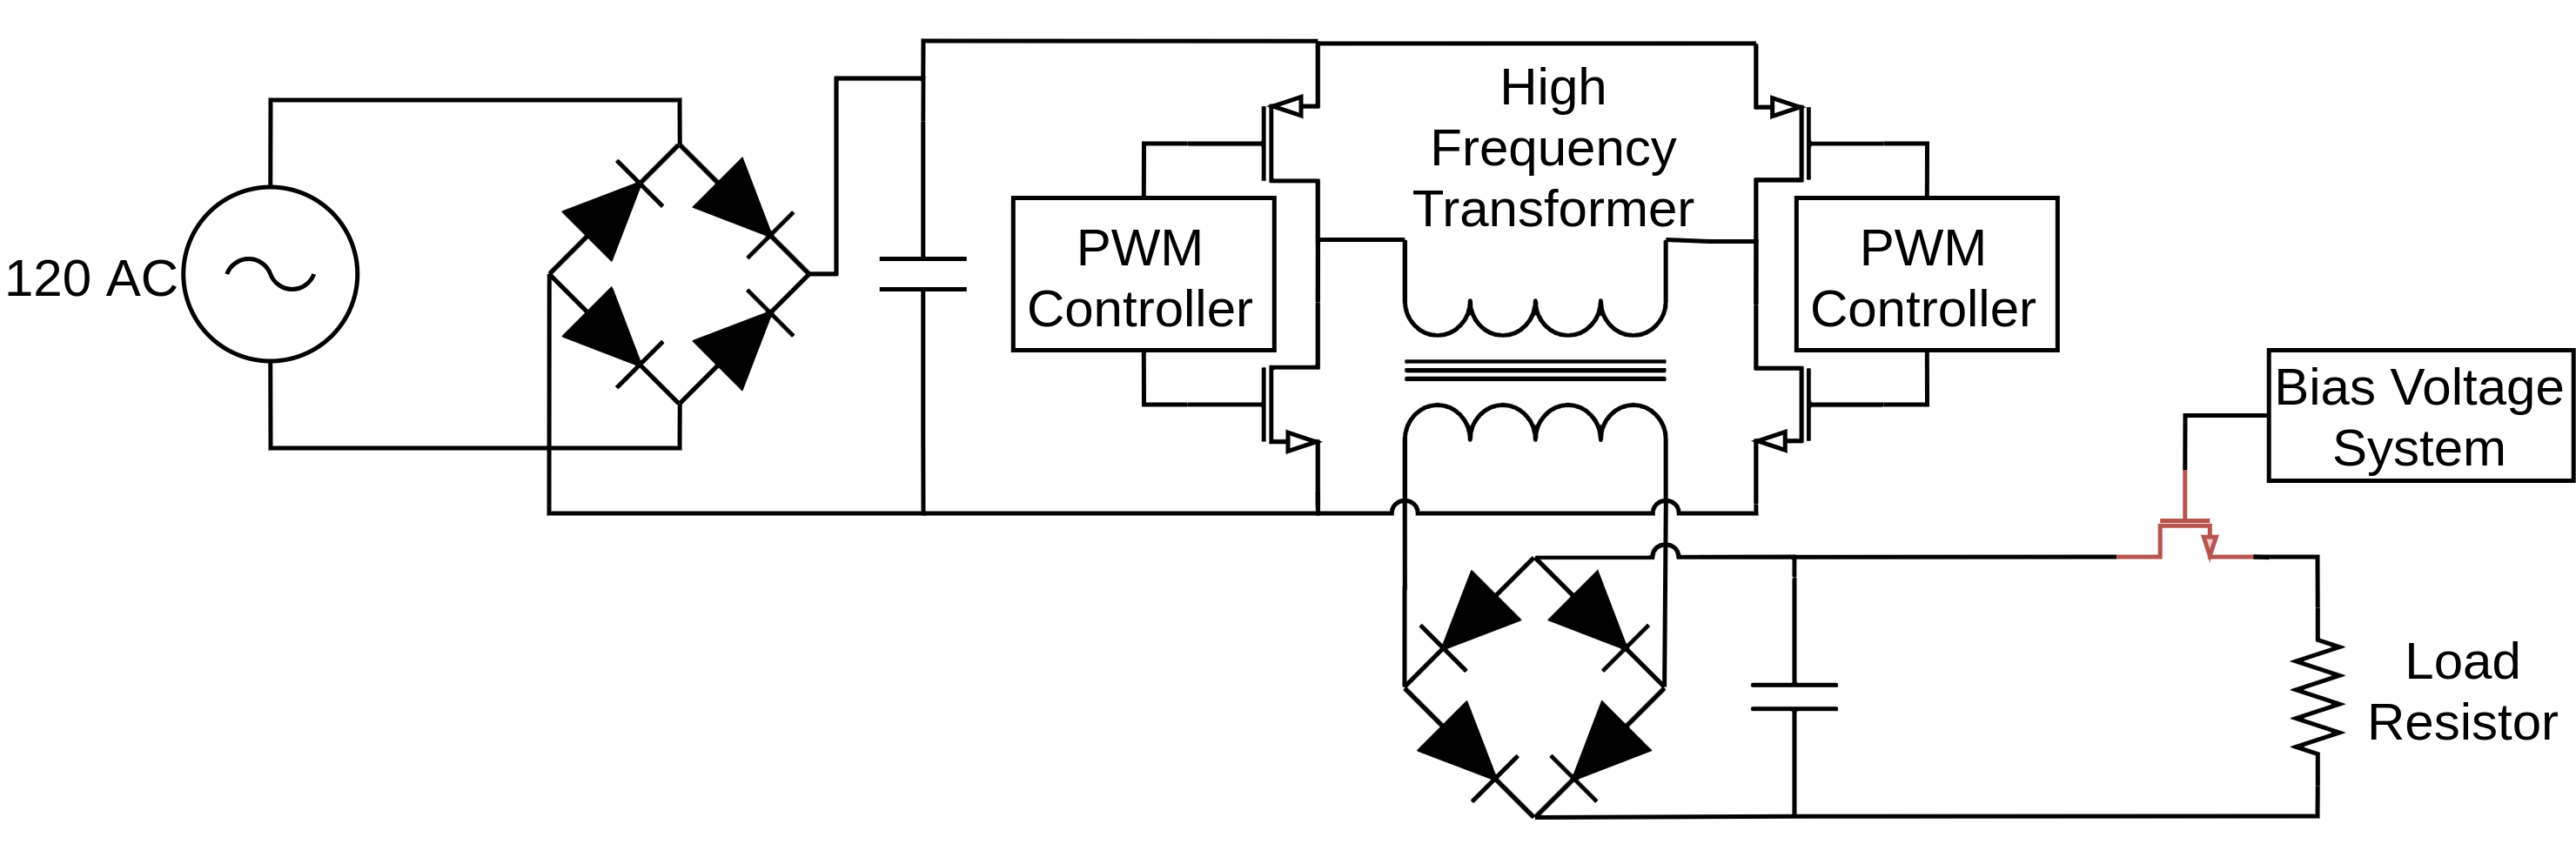
\includegraphics[width=\textwidth]{mixed}
    \caption{Mixed modality design}
    \label{fig:mixed}
\end{figure}
\begin{table}[H]
    \centering
\begin{tabular}{ |c|c||c|c|c|c|  }
    \cline{3-6}
    \multicolumn{1}{c}{}& \multicolumn{1}{c}{}&  \multicolumn{4}{|c|}{\textbf{Options}} \\
    \hline
    \textbf{Criteria} & \textbf{Weight} & Linear & SMPS & Fixed Mixed & Floating Mixed \\ 
    \hline
    Efficiency & 1 & {-}{-}{-} & 0 & {-}{-} & - \\
    Cost & 2 & {-}{-}{-} & 0 & {-} & {-}{-} \\
    Noise & 2 & ++ & 0 & + & + \\
    Step Response & 2 & ++ & 0 & ++ & + \\
    Design Effort & 1 & + & 0 & - & {-}{-} \\ 
    \hline
    \hline
    \multicolumn{2}{|c||}{+} & 9 & 0 & 6 & 4\\
    \multicolumn{2}{|c||}{0} & 0 & 5 & 0 & 0\\
    \multicolumn{2}{|c||}{-} & 9 & 0 & 4 & 7\\
    \hline
    \hline
    \multicolumn{2}{|c||}{\textbf{Net Score}} & 0 & 0 & 2 & -3\\
    \hline
\end{tabular}
\caption{Pugh table for power stage topology selection}
\label{tab:power}
\end{table}

\subsection {Micro-Controller}
Price and USB support were the biggest concern when considering a MCU for the project. 
Four Candidates were considered, and the results are explained below with a summary in 
\autoref{tab:micro}.
The Raspberry PI was not a strong candidate due to its price and lack of ADC/DAC
hardware. The STM32’s tool chain lacks linux support and is not especially intuitive. 
ATmega 2560 lacks USB support which will be important for the communication between 
power supply to PC. The ATmega Samd51 has decent tools and all the required hardware 
at a good price point. In addition to the above mentioned benefits the Samd51 does 
not require many external components making PCB design simpler. A development board 
has been selected for the Samd so that software development may begin before the PCB 
is designed.\\ 
\begin{table}[H]
    \centering
\begin{tabular}{ |c|c||c|c|c|c|  }
    \cline{3-6}
    \multicolumn{1}{c}{}& \multicolumn{1}{c}{}&  \multicolumn{4}{|c|}{\textbf{Options}} \\
    \hline
    \textbf{Criteria} & \textbf{Weight} & ATMega Samd51 & ATMega 2560 & Raspberry Pi & STM32 \\ 
    \hline
    ADC and DAC & 3 & + & 0 & - & + \\
    Price & 5 & + & 0 & - & + \\
    USB support & 5 & + & 0 & + & + \\
    Tools & 2 & 0 & 0 & + & + \\
    Libraries & 1 & - & 0 & + & - \\ 
    \hline
    \hline
    \multicolumn{2}{|c||}{+} & 13 & 0 & 8 & 13\\
    \multicolumn{2}{|c||}{0} & 1 & 5 & 0 & 0\\
    \multicolumn{2}{|c||}{-} & 1 & 0 & 8 & 3\\
    \hline \hline
    \multicolumn{2}{|c||}{\textbf{Net Score}} & 12 & 0 & 0 & 10\\
    \hline
\end{tabular}
\caption{Pugh table for micro-controller selection }
\label{tab:micro}
\end{table}
\section{Management Approach}
\section{Budget}
\section{Timeline}
\section{Facilities}
\section{Disposition Agreement}
\end{document}